\documentclass[border=6pt]{standalone}
\usepackage{lmodern}
\usepackage[T1]{fontenc}
\usepackage{amsmath}
\usepackage{xcolor}
\usepackage{tikz}
\usetikzlibrary{arrows.meta,positioning,decorations.pathreplacing}
\definecolor{cgray}{HTML}{9A9891}
\definecolor{cblue}{HTML}{2F7DC8}
\definecolor{cred}{HTML}{C0392B}
\definecolor{cink}{HTML}{2B2B2B}
\tikzset{
  cell/.style={draw=white,line width=1pt,minimum width=1.35cm,minimum height=0.52cm,inner sep=0pt},
  fitc/.style={cell,fill=cgray!45,text=white,font=\scriptsize},
  calc/.style={cell,fill=cblue,text=white,font=\scriptsize\bfseries},
}
\begin{document}
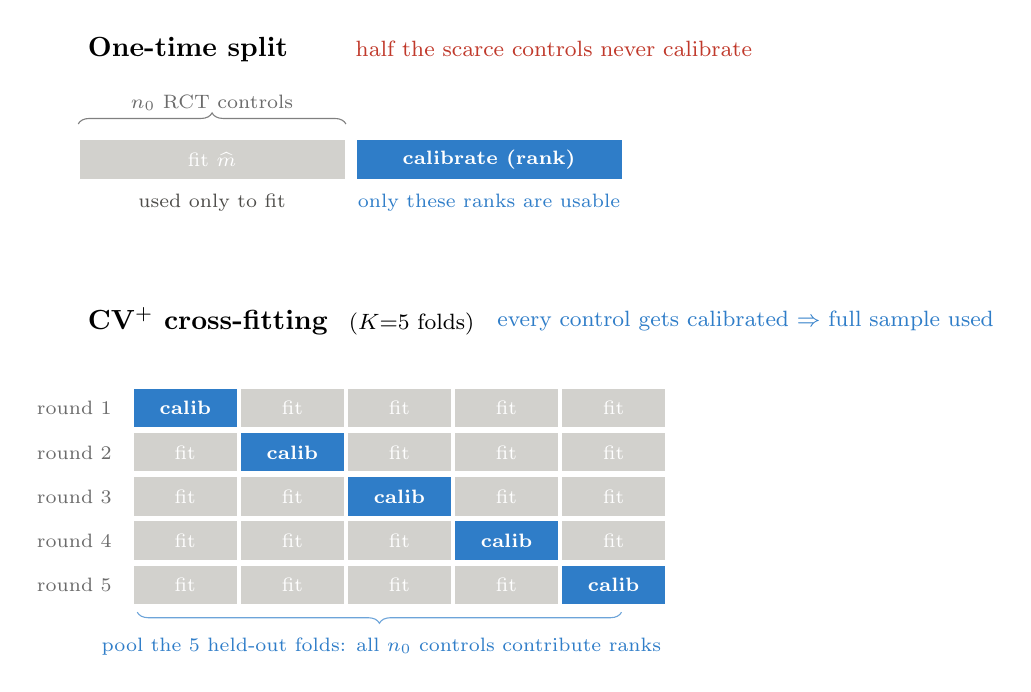
\begin{tikzpicture}[font=\small]

% ================= TOP: one-time split =================
\node[font=\bfseries,anchor=west] at (0,2.1) {One-time split};
\node[font=\footnotesize,text=cred,anchor=west] at (3.4,2.1) {half the scarce controls never calibrate};
\node[fitc,minimum width=3.4cm] (tr) at (1.7,0.7) {fit $\widehat m$};
\node[calc,minimum width=3.4cm,anchor=west] (ca) at (3.5,0.7) {calibrate (rank)};
\node[font=\scriptsize,text=cgray!50!black,below=1pt of tr] {used only to fit};
\node[font=\scriptsize,text=cblue,below=1pt of ca] {only these ranks are usable};
\draw[decorate,decoration={brace,amplitude=4pt},cink!60] (0.0,1.15) -- (3.4,1.15);
\node[font=\scriptsize,text=cink!70] at (1.7,1.42) {$n_0$ RCT controls};

% ================= BOTTOM: CV+ =================
\begin{scope}[yshift=-1.9cm]
\node[font=\bfseries,anchor=west] at (0,0.55) {CV$^+$ cross-fitting \ \mdseries\footnotesize($K{=}5$ folds)};
\node[font=\footnotesize,text=cblue,anchor=west] at (5.2,0.55) {every control gets calibrated $\Rightarrow$ full sample used};
\foreach \r in {1,...,5}{
  \foreach \c in {1,...,5}{
    \pgfmathparse{\c==\r ? "calc" : "fitc"}\edef\st{\pgfmathresult}
    \node[\st] at ({\c*1.36},{-\r*0.56}) {\ifnum\c=\r calib\else fit\fi};
  }
  \node[font=\scriptsize,text=cink!70,anchor=east] at (0.55,{-\r*0.56}) {round \r};
}
\draw[decorate,decoration={brace,amplitude=4pt,mirror},cblue!70]
      (0.75,{-5*0.56-0.35}) -- (6.9,{-5*0.56-0.35});
\node[font=\scriptsize,text=cblue,anchor=north] at (3.85,{-5*0.56-0.55})
      {pool the 5 held-out folds: all $n_0$ controls contribute ranks};
\end{scope}

\end{tikzpicture}
\end{document}
